Nous devons maintenant élaborer des classifieurs pour classer
les imagettes de la base de test dans différentes classes de chiffres.
Nous avons mis en place deux méthodes de classification. La première se 
base sur la distance euclidienne minimale du modèle par rapport à une
imagette de la base de test. La seconde consiste à réaliser la méthode des
$ k $ plus proches voisins. Nous nous sommes exclusivement concentrés sur les taux de réussite en TOP1.

\section{Reconnaissance avec distance euclidienne
minimale sur modèle moyen}

Cette méthode de classification consiste à comparer notre imagette de
test avec le modèle moyen pour chaque classe.
Avec cette méthode, nous obtenons la matrice de confusion suivante.

\begin{figure}[!h]
\centering
\begin{tabular}{|*{11}{c|}}
    \hline
     & 0 & 1 & 2 & 3 & 4 & 5 & 6 & 7 & 8 & 9 \\
    \hline
    0 & 1 & 0  & 0  & 0  & 0  & 0 & 0 & 0 & 0 & 0 \\
    \hline
    1 & 0 & 0.9 & 0.1 & 0  & 0 & 0 & 0 & 0 & 0 & 0 \\
    \hline
    2 & 0 & 0 & 0.9 & 0 & 0 & 0 & 0.1 & 0 & 0 & 0 \\
    \hline
    3 & 0 & 0 & 0 & 0.5 & 0 & 0 & 0 & 0 & 0 & 0.5 \\
    \hline
    4 & 0 & 0 & 0 & 0 & 0.9 & 0 & 0.1 & 0 & 0 & 0 \\
    \hline
    5 & 0 & 0 & 0 & 0 & 0 & 1 & 0 & 0 & 0 & 0 \\
    \hline
    6 & 0 & 0 & 0 & 0 & 0 & 0 & 1 & 0 & 0 & 0 \\
    \hline
    7 & 0 & 0 & 0 & 0.1 & 0 & 0 & 0 & 0.9 & 0 & 0 \\
    \hline
    8 & 0 & 0.2 & 0 & 0 & 0 & 0 & 0 & 0 & 0.8 & 0 \\
    \hline
    9 & 0 & 0 & 0 & 0 & 0 & 0 & 0 & 0.1 & 0.3 & 0.6 \\
    \hline
\end{tabular}
\caption{Matrice de confusion en TOP1 pour cette méthode}
\end{figure} 

Ceci nous donne 85\% de bons résultats avec ce classifieur.

Si nous choisissons en revanche de ne pas utiliser le modèle moyen
pour chaque classe mais, au contraire, d'utiliser la norme euclidienne
sur chaque élément du modèle, nous obtenons un résultat de 92\% en TOP1. Voici 
les résultats pour chaque classe.

\begin{figure}[h!]
\centering
\begin{tabular}{|*{10}{c|}}
    \hline
    0 & 1 & 2 & 3 & 4 & 5 & 6 & 7 & 8 & 9 \\
    \hline
    1 & 1 & 1 & 0.7 & 1 & 1 & 1 & 0.9 & 1 & 0.6  \\
    \hline
\end{tabular}
\caption{Résultat sans moyenner les classes}
\end{figure} 

Nous constatons que les chiffres soulevant le plus de problèmes sont 
le 9 et le 3. Il faudra donc trouver une méthode pour mieux les repérer.

\section{Décision par la méthode des k plus proches voisins}

Grâce au cours de Data-mining, nous savons écrire l'algorithme des k-ppvs.
Mais comment déterminer le nombre de plus proches voisins à sélectionner ?
Nous avons choisi, pour répondre à cette problématique, d'essayer 
avec plusieurs k différents. 

\begin{figure}[h!]
\centering
\begin{tabular}{|*{4}{c|}}
    \hline
    0.92 & 0.93 & 0.90 & 0.91 \\
    \hline
\end{tabular}
\caption{Bons résultats en TOP1 selon la valeur de k (k = 1, 2, 3, 4)}
\end{figure} 

Ceci nous amenant en toute logique à utiliser un k égal à 2.

\section{Méthode des k-ppvs avec d'autres distances}

Pour essayer d'améliorer nos résultats, nous avons voulu essayer
d'utiliser de nouvelles distances. Nous nous sommes donc intéressés
dans un premier temps à la distance de Manhattan. Celle-ci nous donne 
les résultats suivants.

\begin{figure}[h!]
\centering
\begin{tabular}{|*{10}{c|}}
    \hline
    0 & 1 & 2 & 3 & 4 & 5 & 6 & 7 & 8 & 9 \\
    \hline
    1 & 1 & 1 & 0.9 & 0.9 & 1 & 1 & 0.9 & 0.9 & 0.6  \\
    \hline
\end{tabular}
\caption{Résultat avec la distance de Manhattan}
\end{figure} 

Ceci donnant un résultat moyen de 92 \%, ce qui est insuffisant
comparé aux méthodes précédentes.

Nous avons ensuite essayé avec la distance de Minkowski de degré 3.
Celle-ci nous donne les résultats suivants.

\begin{figure}[h!]
\centering
\begin{tabular}{|*{10}{c|}}
    \hline
    0 & 1 & 2 & 3 & 4 & 5 & 6 & 7 & 8 & 9 \\
    \hline
    1 & 1 & 1 & 0.9 & 1 & 1 & 1 & 1 & 0.9 & 0.6  \\
    \hline
\end{tabular}
\caption{Résultat avec la distance de Minkowski}
\end{figure} 

Ceci donnant un résultat moyen de 94 \%, ce qui est déjà un meilleur
résultat. C'est donc très encourageant.

\section{Utilisation d'autres caractéristiques}

A cette étape du projet, nous avons choisi d'utiliser d'autres     
caractéristiques. En effet, les tests réalisés sur les classifieurs
ne montrait pas de grosses améliorations. \\
Nous nous sommes intéressés à la trace. Il s'agit en quelque sorte, 
de réaliser un profil sur un nombre de traits égal au nombre de pixel de
l'image. La figure suivante permet de visualiser les effets de notre
fonction \texttt{traceGD.m}.

\begin{figure}[h!]
\centering
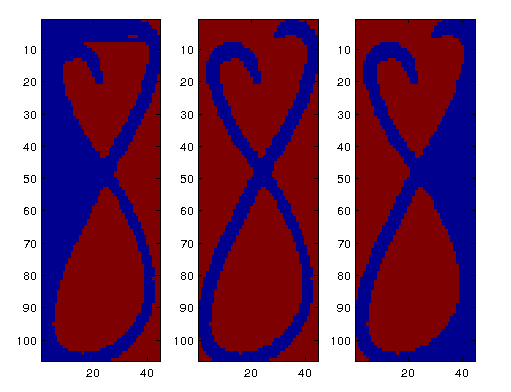
\includegraphics[scale=0.5]{trace.png}
\caption{Exemples de résultats de la fonction trace}
\end{figure}

Les résultats avec cette caractéristique sont les suivants :

\begin{figure}[h!]
\centering
\begin{tabular}{|*{2}{c|}}
    \hline
    kppv/trace Gauche & 0.88 \\
    \hline
    DEG/trace Gauche & 0.87 \\
    \hline
    kppv/trace Droite & 0.93 \\
    \hline
    DEG/trace Droite & 0.93 \\
    \hline
\end{tabular}
\caption{Taux de bons résultats avec la caractéristique trace}
\end{figure}

Nous avons aussi réalisé une méthode de classification par les kppvs
avec l'utilisation d'une trace Gauche-Droite qui donne des résultats 
peu intéressants mais qui reconnaît bien les 9. Il s'agirait donc de 
l'utiliser avec un classifieur plus efficace pour obtenir un très bon
taux de reconnaissance.

\section{Combinaison de classifieurs}

Nous allons donc essayer de combiner les classifieurs kppv/Minkowski3 avec la 
DEG/trace Droite et la DEG/trace Gauche-Droite. Nous choisirons les
paramètres optimaux dans le maximum de cas. \\
La combinaison de ces classifieurs commence par les classifieurs les plus
précis pour terminer avec le moins efficace mais qui discrimine mieux 
les 9 des 8. \\
Dans chaque cas, on vérifiera si le résultat obtenu est certain avec le classifieur utilisé.\\
S'il ne l'est pas, on passe au classifieur suivant pour essayer de déterminer avec exactitude la classe.

\section{Résultats finaux}

L'utilisation d'une combinaison de classifieurs nous a permis d'obtenir
de très bons résultats. En effet, nous avons réussi à obtenir un
taux de bonnes réponses de 98\%, voir le vecteur de résultat suivant.

\begin{figure}[h!]
\centering
\begin{tabular}{|*{10}{c|}}
    \hline
    0 & 1 & 2 & 3 & 4 & 5 & 6 & 7 & 8 & 9 \\
    \hline
    1 & 1 & 1 & 0.9 & 1 & 1 & 1 & 1 & 0.9 & 1  \\
    \hline
\end{tabular}
\caption{Résultat des classifieurs combinés}
\end{figure} 

Les confusions restantes sont obtenues sur un 3 et un 8 que notre
chaîne de reconnaissance de formes confond avec des 9. 
